\section{Численный метод Брауна--Робинсон}

Метод Брауна—Робинсона является итерационным численным методом для приближенного
нахождения решения матричных антагонистических игр. Этот метод позволяет находить
оптимальные стратегии игроков в смешанных стратегиях, постепенно улучшая оценки
верхней и нижней цены игры.

Метод заключается в последовательном обновлении частот выбора стратегий игроками.
На каждом шаге $k$ игроки выбирают стратегии, основываясь на накопленной статистике выигрышей:

Первый игрок выбирает стратегию, максимизирующую ожидаемый выигрыш, исходя из наблюденных
действий второго игрока.

Второй игрок выбирает стратегию, минимизирующую ожидаемый выигрыш первого игрока.

Оценки верхней и нижней границы цены игры вычисляются по формулам:

\begin{equation}
  \overline{v}[k] = \max_{i \in A} \sum_{j \in B} c_{ij} \tilde{y}_j[k],
\end{equation}
\begin{equation}
  \underline{v}[k] = \min{\sum_{i \in A} c_{ij} \tilde{x}_i[k]}.
\end{equation}

Средние значения этих оценок используются для приближенного вычисления цены игры.
Процесс продолжается до достижения заданной точности $\varepsilon \leq 0.1$.

На таблице~\ref{tab:tab1} представлена таблица итеративного алгоритма Брауна--Робинсон
для решения исходной матричной игры. Для решения всего потребовалось 108 итераций.

\begin{longtable}[H]{c|c|c|c|c|c|c|c|c|c|c|c|}
    \caption{Результаты итерационного процесса с указанием стратегий
     и стоимостей игры}\label{tab:tab1}\\ \hline
    \endfirsthead
    \caption*{Продолжение таблицы \ref{tab:tab1}}\\ \hline
    \endhead
    \hline
    \endfoot
    \hline
    \endlastfoot
    \# & a & b & $x_1$ & $x_2$ & $x_3$ & $y_1$ & $y_2$ & $y_3$ & Верх. & Ниж. & $\varepsilon$ \\ \hline
    1 & $x_1$ & $y_1$ & 11 & 16 & 15 & 11 & 10 & 15 & 16.000 & 10.000 & 6.000 \\ \hline
    2 & $x_2$ & $y_2$ & 21 & 21 & 35 & 27 & 15 & 28 & 17.500 & 7.500 & 6.000 \\ \hline
    3 & $x_3$ & $y_2$ & 31 & 26 & 55 & 42 & 35 & 38 & 18.333 & 11.667 & 4.333 \\ \hline
    4 & $x_3$ & $y_2$ & 41 & 31 & 75 & 57 & 55 & 48 & 18.750 & 12.000 & 4.000 \\ \hline
    5 & $x_3$ & $y_3$ & 56 & 44 & 85 & 72 & 75 & 58 & 17.000 & 11.600 & 4.000 \\ \hline
    6 & $x_3$ & $y_3$ & 71 & 57 & 95 & 87 & 95 & 68 & 15.833 & 11.333 & 3.833 \\ \hline
    7 & $x_3$ & $y_3$ & 86 & 70 & 105 & 102 & 115 & 78 & 15.000 & 11.143 & 3.000 \\ \hline
    8 & $x_3$ & $y_3$ & 101 & 83 & 115 & 117 & 135 & 88 & 14.375 & 11.000 & 2.375 \\ \hline
    9 & $x_3$ & $y_3$ & 116 & 96 & 125 & 132 & 155 & 98 & 13.889 & 10.889 & 1.889 \\ \hline
    10 & $x_3$ & $y_3$ & 131 & 109 & 135 & 147 & 175 & 108 & 13.500 & 10.800 & 1.500 \\ \hline
    11 & $x_3$ & $y_3$ & 146 & 122 & 145 & 162 & 195 & 118 & 13.273 & 10.727 & 1.273 \\ \hline
    12 & $x_1$ & $y_3$ & 161 & 135 & 155 & 173 & 205 & 133 & 13.417 & 11.083 & 1.273 \\ \hline
    13 & $x_1$ & $y_3$ & 176 & 148 & 165 & 184 & 215 & 148 & 13.538 & 11.385 & 1.273 \\ \hline
    14 & $x_1$ & $y_3$ & 191 & 161 & 175 & 195 & 225 & 163 & 13.643 & 11.643 & 1.273 \\ \hline
    15 & $x_1$ & $y_3$ & 206 & 174 & 185 & 206 & 235 & 178 & 13.733 & 11.867 & 1.273 \\ \hline
    16 & $x_1$ & $y_3$ & 221 & 187 & 195 & 217 & 245 & 193 & 13.812 & 12.062 & 1.210 \\ \hline
    17 & $x_1$ & $y_3$ & 236 & 200 & 205 & 228 & 255 & 208 & 13.882 & 12.235 & 1.037 \\ \hline
    18 & $x_1$ & $y_3$ & 251 & 213 & 215 & 239 & 265 & 223 & 13.944 & 12.389 & 0.884 \\ \hline
    19 & $x_1$ & $y_3$ & 266 & 226 & 225 & 250 & 275 & 238 & 14.000 & 12.526 & 0.746 \\ \hline
    20 & $x_1$ & $y_3$ & 281 & 239 & 235 & 261 & 285 & 253 & 14.050 & 12.650 & 0.623 \\ \hline
    21 & $x_1$ & $y_3$ & 296 & 252 & 245 & 272 & 295 & 268 & 14.095 & 12.762 & 0.511 \\ \hline
    22 & $x_1$ & $y_3$ & 311 & 265 & 255 & 283 & 305 & 283 & 14.136 & 12.864 & 0.409 \\ \hline
    23 & $x_1$ & $y_3$ & 326 & 278 & 265 & 294 & 315 & 298 & 14.174 & 12.783 & 0.409 \\ \hline
    24 & $x_1$ & $y_1$ & 337 & 294 & 280 & 305 & 325 & 313 & 14.042 & 12.708 & 0.409 \\ \hline
    25 & $x_1$ & $y_1$ & 348 & 310 & 295 & 316 & 335 & 328 & 13.920 & 12.640 & 0.409 \\ \hline
    26 & $x_1$ & $y_1$ & 359 & 326 & 310 & 327 & 345 & 343 & 13.808 & 12.577 & 0.409 \\ \hline
    27 & $x_1$ & $y_1$ & 370 & 342 & 325 & 338 & 355 & 358 & 13.704 & 12.519 & 0.409 \\ \hline
    28 & $x_1$ & $y_1$ & 381 & 358 & 340 & 349 & 365 & 373 & 13.607 & 12.464 & 0.409 \\ \hline
    29 & $x_1$ & $y_1$ & 392 & 374 & 355 & 360 & 375 & 388 & 13.517 & 12.414 & 0.409 \\ \hline
    30 & $x_1$ & $y_1$ & 403 & 390 & 370 & 371 & 385 & 403 & 13.433 & 12.367 & 0.409 \\ \hline
    31 & $x_1$ & $y_1$ & 414 & 406 & 385 & 382 & 395 & 418 & 13.355 & 12.323 & 0.409 \\ \hline
    32 & $x_1$ & $y_1$ & 425 & 422 & 400 & 393 & 405 & 433 & 13.281 & 12.281 & 0.409 \\ \hline
    33 & $x_1$ & $y_1$ & 436 & 438 & 415 & 404 & 415 & 448 & 13.273 & 12.242 & 0.409 \\ \hline
    34 & $x_2$ & $y_1$ & 447 & 454 & 430 & 420 & 420 & 461 & 13.353 & 12.353 & 0.409 \\ \hline
    35 & $x_2$ & $y_2$ & 457 & 459 & 450 & 436 & 425 & 474 & 13.114 & 12.143 & 0.251 \\ \hline
    36 & $x_2$ & $y_2$ & 467 & 464 & 470 & 452 & 430 & 487 & 13.056 & 11.944 & 0.192 \\ \hline
    37 & $x_3$ & $y_2$ & 477 & 469 & 490 & 467 & 450 & 497 & 13.243 & 12.162 & 0.192 \\ \hline
    38 & $x_3$ & $y_2$ & 487 & 474 & 510 & 482 & 470 & 507 & 13.421 & 12.368 & 0.192 \\ \hline
    39 & $x_3$ & $y_2$ & 497 & 479 & 530 & 497 & 490 & 517 & 13.590 & 12.564 & 0.192 \\ \hline
    40 & $x_3$ & $y_2$ & 507 & 484 & 550 & 512 & 510 & 527 & 13.750 & 12.750 & 0.192 \\ \hline
    41 & $x_3$ & $y_2$ & 517 & 489 & 570 & 527 & 530 & 537 & 13.902 & 12.854 & 0.192 \\ \hline
    42 & $x_3$ & $y_1$ & 528 & 505 & 585 & 542 & 550 & 547 & 13.929 & 12.905 & 0.151 \\ \hline
    43 & $x_3$ & $y_1$ & 539 & 521 & 600 & 557 & 570 & 557 & 13.953 & 12.953 & 0.102 \\ \hline
    44 & $x_3$ & $y_1$ & 550 & 537 & 615 & 572 & 590 & 567 & 13.977 & 12.886 & 0.102 \\ \hline
    45 & $x_3$ & $y_3$ & 565 & 550 & 625 & 587 & 610 & 577 & 13.889 & 12.822 & 0.102 \\ \hline
    46 & $x_3$ & $y_3$ & 580 & 563 & 635 & 602 & 630 & 587 & 13.804 & 12.761 & 0.102 \\ \hline
    47 & $x_3$ & $y_3$ & 595 & 576 & 645 & 617 & 650 & 597 & 13.723 & 12.702 & 0.102 \\ \hline
    48 & $x_3$ & $y_3$ & 610 & 589 & 655 & 632 & 670 & 607 & 13.646 & 12.646 & 0.102 \\ \hline
    49 & $x_3$ & $y_3$ & 625 & 602 & 665 & 647 & 690 & 617 & 13.571 & 12.592 & 0.102 \\ \hline
    50 & $x_3$ & $y_3$ & 640 & 615 & 675 & 662 & 710 & 627 & 13.500 & 12.540 & 0.102 \\ \hline
    51 & $x_3$ & $y_3$ & 655 & 628 & 685 & 677 & 730 & 637 & 13.431 & 12.490 & 0.102 \\ \hline
    52 & $x_3$ & $y_3$ & 670 & 641 & 695 & 692 & 750 & 647 & 13.365 & 12.442 & 0.102 \\ \hline
    53 & $x_3$ & $y_3$ & 685 & 654 & 705 & 707 & 770 & 657 & 13.302 & 12.396 & 0.102 \\ \hline
    54 & $x_3$ & $y_3$ & 700 & 667 & 715 & 722 & 790 & 667 & 13.241 & 12.352 & 0.102 \\ \hline
    55 & $x_3$ & $y_3$ & 715 & 680 & 725 & 737 & 810 & 677 & 13.182 & 12.309 & 0.102 \\ \hline
    56 & $x_3$ & $y_3$ & 730 & 693 & 735 & 752 & 830 & 687 & 13.125 & 12.268 & 0.102 \\ \hline
    57 & $x_3$ & $y_3$ & 745 & 706 & 745 & 767 & 850 & 697 & 13.070 & 12.228 & 0.102 \\ \hline
    58 & $x_3$ & $y_3$ & 760 & 719 & 755 & 782 & 870 & 707 & 13.103 & 12.190 & 0.102 \\ \hline
    59 & $x_1$ & $y_3$ & 775 & 732 & 765 & 793 & 880 & 722 & 13.136 & 12.237 & 0.102 \\ \hline
    60 & $x_1$ & $y_3$ & 790 & 745 & 775 & 804 & 890 & 737 & 13.167 & 12.283 & 0.102 \\ \hline
    61 & $x_1$ & $y_3$ & 805 & 758 & 785 & 815 & 900 & 752 & 13.197 & 12.328 & 0.102 \\ \hline
    62 & $x_1$ & $y_3$ & 820 & 771 & 795 & 826 & 910 & 767 & 13.226 & 12.371 & 0.102 \\ \hline
    63 & $x_1$ & $y_3$ & 835 & 784 & 805 & 837 & 920 & 782 & 13.254 & 12.413 & 0.102 \\ \hline
    64 & $x_1$ & $y_3$ & 850 & 797 & 815 & 848 & 930 & 797 & 13.281 & 12.453 & 0.102 \\ \hline
    65 & $x_1$ & $y_3$ & 865 & 810 & 825 & 859 & 940 & 812 & 13.308 & 12.492 & 0.102 \\ \hline
    66 & $x_1$ & $y_3$ & 880 & 823 & 835 & 870 & 950 & 827 & 13.333 & 12.530 & 0.102 \\ \hline
    67 & $x_1$ & $y_3$ & 895 & 836 & 845 & 881 & 960 & 842 & 13.358 & 12.567 & 0.102 \\ \hline
    68 & $x_1$ & $y_3$ & 910 & 849 & 855 & 892 & 970 & 857 & 13.382 & 12.603 & 0.102 \\ \hline
    69 & $x_1$ & $y_3$ & 925 & 862 & 865 & 903 & 980 & 872 & 13.406 & 12.638 & 0.102 \\ \hline
    70 & $x_1$ & $y_3$ & 940 & 875 & 875 & 914 & 990 & 887 & 13.429 & 12.671 & 0.102 \\ \hline
    71 & $x_1$ & $y_3$ & 955 & 888 & 885 & 925 & 1000 & 902 & 13.451 & 12.704 & 0.102 \\ \hline
    72 & $x_1$ & $y_3$ & 970 & 901 & 895 & 936 & 1010 & 917 & 13.472 & 12.736 & 0.102 \\ \hline
    73 & $x_1$ & $y_3$ & 985 & 914 & 905 & 947 & 1020 & 932 & 13.493 & 12.767 & 0.102 \\ \hline
    74 & $x_1$ & $y_3$ & 1000 & 927 & 915 & 958 & 1030 & 947 & 13.514 & 12.797 & 0.102 \\ \hline
    75 & $x_1$ & $y_3$ & 1015 & 940 & 925 & 969 & 1040 & 962 & 13.533 & 12.827 & 0.102 \\ \hline
    76 & $x_1$ & $y_3$ & 1030 & 953 & 935 & 980 & 1050 & 977 & 13.553 & 12.855 & 0.102 \\ \hline
    77 & $x_1$ & $y_3$ & 1045 & 966 & 945 & 991 & 1060 & 992 & 13.571 & 12.870 & 0.102 \\ \hline
    78 & $x_1$ & $y_1$ & 1056 & 982 & 960 & 1002 & 1070 & 1007 & 13.538 & 12.846 & 0.102 \\ \hline
    79 & $x_1$ & $y_1$ & 1067 & 998 & 975 & 1013 & 1080 & 1022 & 13.506 & 12.823 & 0.102 \\ \hline
    80 & $x_1$ & $y_1$ & 1078 & 1014 & 990 & 1024 & 1090 & 1037 & 13.475 & 12.800 & 0.102 \\ \hline
    81 & $x_1$ & $y_1$ & 1089 & 1030 & 1005 & 1035 & 1100 & 1052 & 13.444 & 12.778 & 0.102 \\ \hline
    82 & $x_1$ & $y_1$ & 1100 & 1046 & 1020 & 1046 & 1110 & 1067 & 13.415 & 12.756 & 0.102 \\ \hline
    83 & $x_1$ & $y_1$ & 1111 & 1062 & 1035 & 1057 & 1120 & 1082 & 13.386 & 12.735 & 0.102 \\ \hline
    84 & $x_1$ & $y_1$ & 1122 & 1078 & 1050 & 1068 & 1130 & 1097 & 13.357 & 12.714 & 0.102 \\ \hline
    85 & $x_1$ & $y_1$ & 1133 & 1094 & 1065 & 1079 & 1140 & 1112 & 13.329 & 12.694 & 0.102 \\ \hline
    86 & $x_1$ & $y_1$ & 1144 & 1110 & 1080 & 1090 & 1150 & 1127 & 13.302 & 12.674 & 0.102 \\ \hline
    87 & $x_1$ & $y_1$ & 1155 & 1126 & 1095 & 1101 & 1160 & 1142 & 13.276 & 12.655 & 0.102 \\ \hline
    88 & $x_1$ & $y_1$ & 1166 & 1142 & 1110 & 1112 & 1170 & 1157 & 13.250 & 12.636 & 0.102 \\ \hline
    89 & $x_1$ & $y_1$ & 1177 & 1158 & 1125 & 1123 & 1180 & 1172 & 13.225 & 12.618 & 0.102 \\ \hline
    90 & $x_1$ & $y_1$ & 1188 & 1174 & 1140 & 1134 & 1190 & 1187 & 13.200 & 12.600 & 0.102 \\ \hline
    91 & $x_1$ & $y_1$ & 1199 & 1190 & 1155 & 1145 & 1200 & 1202 & 13.176 & 12.582 & 0.102 \\ \hline
    92 & $x_1$ & $y_1$ & 1210 & 1206 & 1170 & 1156 & 1210 & 1217 & 13.152 & 12.565 & 0.102 \\ \hline
    93 & $x_1$ & $y_1$ & 1221 & 1222 & 1185 & 1167 & 1220 & 1232 & 13.140 & 12.548 & 0.102 \\ \hline
    94 & $x_2$ & $y_1$ & 1232 & 1238 & 1200 & 1183 & 1225 & 1245 & 13.170 & 12.585 & 0.102 \\ \hline
    95 & $x_2$ & $y_1$ & 1243 & 1254 & 1215 & 1199 & 1230 & 1258 & 13.200 & 12.621 & 0.102 \\ \hline
    96 & $x_2$ & $y_1$ & 1254 & 1270 & 1230 & 1215 & 1235 & 1271 & 13.229 & 12.656 & 0.102 \\ \hline
    97 & $x_2$ & $y_1$ & 1265 & 1286 & 1245 & 1231 & 1240 & 1284 & 13.258 & 12.691 & 0.102 \\ \hline
    98 & $x_2$ & $y_1$ & 1276 & 1302 & 1260 & 1247 & 1245 & 1297 & 13.286 & 12.704 & 0.102 \\ \hline
    99 & $x_2$ & $y_2$ & 1286 & 1307 & 1280 & 1263 & 1250 & 1310 & 13.202 & 12.626 & 0.102 \\ \hline
    100 & $x_2$ & $y_2$ & 1296 & 1312 & 1300 & 1279 & 1255 & 1323 & 13.120 & 12.550 & 0.102 \\ \hline
    101 & $x_2$ & $y_2$ & 1306 & 1317 & 1320 & 1295 & 1260 & 1336 & 13.069 & 12.475 & 0.102 \\ \hline
    102 & $x_3$ & $y_2$ & 1316 & 1322 & 1340 & 1310 & 1280 & 1346 & 13.137 & 12.549 & 0.102 \\ \hline
    103 & $x_3$ & $y_2$ & 1326 & 1327 & 1360 & 1325 & 1300 & 1356 & 13.204 & 12.621 & 0.102 \\ \hline
    104 & $x_3$ & $y_2$ & 1336 & 1332 & 1380 & 1340 & 1320 & 1366 & 13.269 & 12.692 & 0.102 \\ \hline
    105 & $x_3$ & $y_2$ & 1346 & 1337 & 1400 & 1355 & 1340 & 1376 & 13.333 & 12.762 & 0.102 \\ \hline
    106 & $x_3$ & $y_2$ & 1356 & 1342 & 1420 & 1370 & 1360 & 1386 & 13.396 & 12.830 & 0.102 \\ \hline
    107 & $x_3$ & $y_2$ & 1366 & 1347 & 1440 & 1385 & 1380 & 1396 & 13.458 & 12.897 & 0.102 \\ \hline
    108 & $x_3$ & $y_2$ & 1376 & 1352 & 1460 & 1400 & 1400 & 1406 & 13.519 & 12.963 & 0.093 \\ \hline
\end{longtable}

Алгоритм остановился, так как значение $\varepsilon$ стало меньше 0.1. Значит ответом будут являться
значения, представленные на рисунке~\ref{fig:fig3}.

\begin{figure}
  \centering
  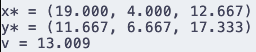
\includegraphics[scale=0.7]{../../artifacts/lw1/brown_robinson_solution.png}
  \caption{Ответ для задачи, посчитанный алгоритмом Брауна--Робинсон}
  \label{fig:fig3}
\end{figure}
